\documentclass[answers]{exam}
\usepackage[english]{babel}
\usepackage[utf8x]{inputenc}
\usepackage{amsmath,amssymb,amsthm}

\title{OPER 510 - Introduction to Mathematical Programming%
	\\ Assignment 5}
\author{Brandon Hosley}
\date{\today}

\usepackage[table,dvipsnames]{xcolor}
\usepackage{graphicx}
\usepackage{enumitem}

\usepackage{booktabs}

\usepackage{tabularx,makecell,diagbox}
\newcolumntype{Y}{>{\centering\arraybackslash}X}

\usepackage{pgf,tikz,tikz-3dplot}
\usetikzlibrary{shapes,arrows,positioning,backgrounds}
\tikzset{%
roundnode/.style={circle, draw=MidnightBlue!90, thick, fill=gray!40},
pt/.style={draw=MidnightBlue, thick,->,>=stealth',shorten >=1pt},
fwd/.style={preaction={draw=YellowOrange,-, line width=2pt,shorten >=3pt}}
}



\usepackage{float}

\begin{document}
\maketitle
\unframedsolutions

\begin{questions}
\question
Find the shortest path from node 1 to node 6 in Figure 3.

\includegraphics[width=0.9\linewidth]{"Screenshot 2022-11-24 at 12.10.09 PM"}

\begin{solution} \\
	\begin{tabular}{ccccccc}
		From: &  1  &  2  &  3  &  4  & 5 & 6 \\ \midrule
		 To:  &  6  &  6  &  6  &  6  & 6 & 6 \\
		Min:  & 44* & 31* & 21* & 12* & 7 & 0
	\end{tabular} \hspace{6ex} \medskip
	\( 4 \rightarrow \begin{cases}
		6 &= 12 \\
		5 &= 7+7=14
	\end{cases} \) \\
	\begin{tabular}{ccccccc}
		From: &  1  &  2  &  3  & 4  & 5 & 6 \\ \midrule
		 To:  &  6  &  6  &  6  & 6  & 6 & 6 \\
		Min:  & 44* & 31* & 21* & 12 & 7 & 0
	\end{tabular} \hspace{7.25ex} \smallskip
	\( 3 \rightarrow \begin{cases}
		6 &= 21 \\
		5 &= 12+7=19 \\
		4 &= 7+12=19
	\end{cases} \) \\
	\begin{tabular}{ccccccc}
		From: &  1  & 2  &  3  & 4  & 5 & 6 \\ \midrule
		 To:  &  6  & 4  & 4,5 & 6  & 6 & 6 \\
		Min:  & 44* & 24 & 19  & 12 & 7 & 0
	\end{tabular} \hspace{9ex}
	\( 2 \rightarrow \begin{cases}
		6 &= 31 \\
		5 &= 21+7=28 \\
		4 &= 12+12=24 \\
		3 &= 7+19=26
	\end{cases} \) \\
	\begin{tabular}{ccccccc}
		From: &  1  & 2  &  3  & 4  & 5 & 6 \\ \midrule
		 To:  & 2,3 & 4  & 4,5 & 6  & 6 & 6 \\
		Min:  & 31  & 24 & 19  & 12 & 7 & 0
	\end{tabular} \hspace{9.5ex}
	\( 1 \rightarrow \begin{cases}
		6 &= 44 \\
		5 &= 31+7=38 \\
		4 &= 21+12=33 \\
		3 &= 12+19=31 \\
		2 &= 7+24=31
	\end{cases} \) \\
	
	\textbf{Summary: }	
	There are multiple shortest paths, branching at node one and node three.
	1-2-4-6,
	1-3-4-6, and
	1-3-5-6 are all 31 unit cost in weight.
	

\end{solution}

\clearpage

\question
Figures 18–20 show the networks for Problems 1–3. Find the maximum flow from source to sink in each network. Find a cut in the network whose capacity equals the
maximum flow in the network. Also, set up an LP that could be used to determine the maximum flow in the network.

\includegraphics[width=\linewidth]{"Screenshot 2022-11-24 at 12.23.30 PM"}

\begin{solution}	
\begin{figure}[H]
	\centering
	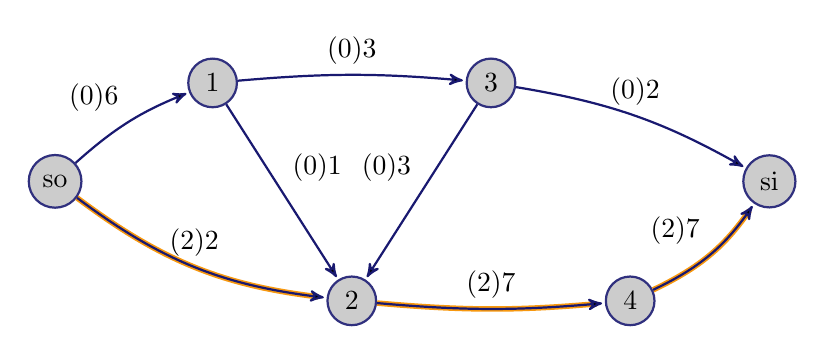
\begin{tikzpicture}[node distance=2.5cm]		
		\node[roundnode] (source) {so};
		\node[roundnode] (one) [right of=source, xshift=-0.5cm, yshift=1.25cm] {1};
		\node[roundnode] (two) [below right of=one, yshift=-1cm] {2};
		\node[roundnode] (three) [above right of=two, yshift=1cm] {3};
		\node[roundnode] (four) [below right of=three,yshift=-1cm] {4};
		\node[roundnode] (sink) [above right of=four, yshift=-0.25cm] {si};
		
		\path[pt] (source) 	edge [bend left=10]  node [above left] 	{(0)6} (one);
		\draw[pt] (source) 	edge [bend right=15, fwd] node [above] 	{(2)2} (two);
		\path[pt] (one) 	edge 	node [above right]			{(0)1} (two);
		\path[pt] (one) 	edge [bend left=5]   node [above] 	{(0)3} (three);
		\path[pt] (three) 	edge 	node [above left] 			{(0)3} (two);
		\path[pt] (two) 	edge [bend right=5, fwd]  node [above] 	{(2)7} (four);
		\path[pt] (three) 	edge [bend left=10]  node [above] 	{(0)2} (sink);
		\path[pt] (four) 	edge [bend right=15,fwd] node [above left] 	{(2)7} (sink);
	\end{tikzpicture}
	\caption{Forward Pass 1}
\end{figure}
\begin{figure}[H]
	\centering
	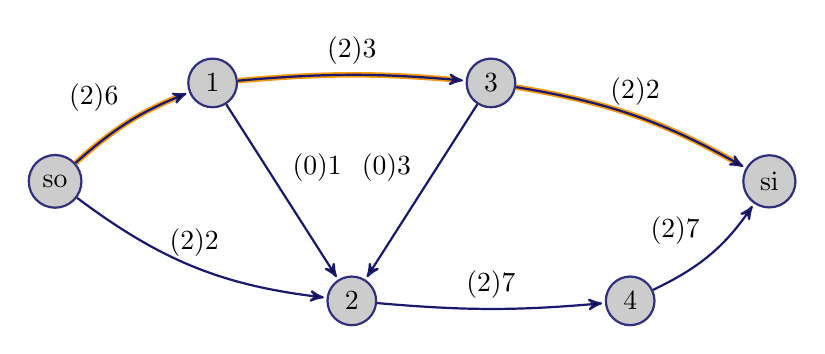
\begin{tikzpicture}[node distance=2.5cm]		
		\node[roundnode] (source) {so};
		\node[roundnode] (one) [right of=source, xshift=-0.5cm, yshift=1.25cm] {1};
		\node[roundnode] (two) [below right of=one, yshift=-1cm] {2};
		\node[roundnode] (three) [above right of=two, yshift=1cm] {3};
		\node[roundnode] (four) [below right of=three,yshift=-1cm] {4};
		\node[roundnode] (sink) [above right of=four, yshift=-0.25cm] {si};
		
		\path[pt] (source) edge [bend left=10,fwd] node [above left] {(2)6} (one);
		\path[pt] (source) 	edge [bend right=15] node [above] 		{(2)2} (two);
		\path[pt] (one) 	edge 	node [above right]				{(0)1} (two);
		\path[pt] (one) 	edge [bend left=5,fwd]   node [above] 		{(2)3} (three);
		\path[pt] (three) 	edge 	node [above left] 				{(0)3} (two);
		\path[pt] (two) 	edge [bend right=5]  node [above] 		{(2)7} (four);
		\path[pt] (three) 	edge [bend left=10,fwd]  node [above] 		{(2)2} (sink);
		\path[pt] (four) 	edge [bend right=15] node [above left] 	{(2)7} (sink);
	\end{tikzpicture}
	\caption{Forward Pass 2}
\end{figure}
\begin{figure}[H]
	\centering
	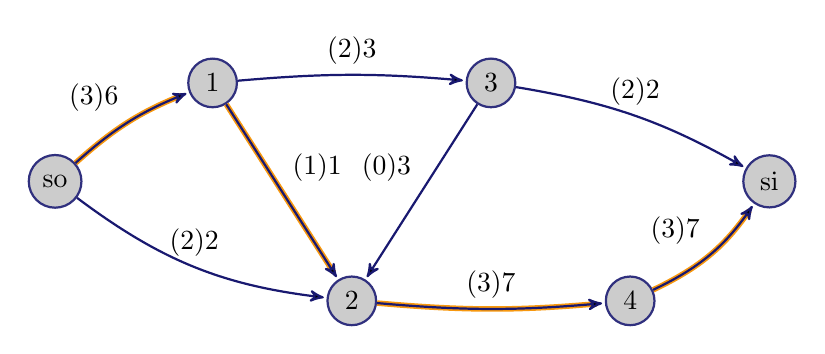
\begin{tikzpicture}[node distance=2.5cm]		
		\node[roundnode] (source) {so};
		\node[roundnode] (one) [right of=source, xshift=-0.5cm, yshift=1.25cm] {1};
		\node[roundnode] (two) [below right of=one, yshift=-1cm] {2};
		\node[roundnode] (three) [above right of=two, yshift=1cm] {3};
		\node[roundnode] (four) [below right of=three,yshift=-1cm] {4};
		\node[roundnode] (sink) [above right of=four, yshift=-0.25cm] {si};
		
		\path[pt] (source) 	edge [bend left=10,fwd]  node [above left] 	{(3)6} (one);
		\path[pt] (source) 	edge [bend right=15] node [above] 		{(2)2} (two);
		\path[pt] (one) 	edge [fwd]	node [above right]				{(1)1} (two);
		\path[pt] (one) 	edge [bend left=5]   node [above] 		{(2)3} (three);
		\path[pt] (three) 	edge 	node [above left] 				{(0)3} (two);
		\path[pt] (two) 	edge [bend right=5,fwd]  node [above] 		{(3)7} (four);
		\path[pt] (three) 	edge [bend left=10]  node [above] 		{(2)2} (sink);
		\path[pt] (four) 	edge [bend right=15,fwd] node [above left] 	{(3)7} (sink);
	\end{tikzpicture}
	\caption{Forward Pass 3}
\end{figure}
\begin{figure}[H]
	\centering
	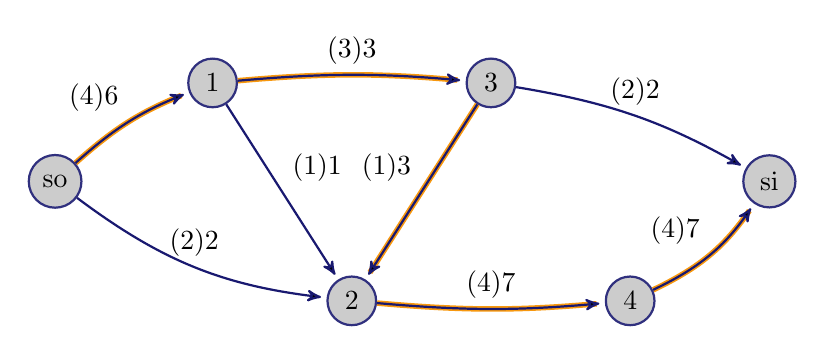
\begin{tikzpicture}[->,>=stealth',shorten >=2pt,
		line width=0/5pt,node distance=2.5cm,
		roundnode/.style={circle, draw=MidnightBlue!90, thick, fill=gray!40},
		pt/.style={draw=MidnightBlue, thick},
		pts/.style={draw=MidnightBlue, thick}]		
		\node[roundnode] (source) {so};
		\node[roundnode] (one) [right of=source, xshift=-0.5cm, yshift=1.25cm] {1};
		\node[roundnode] (two) [below right of=one, yshift=-1cm] {2};
		\node[roundnode] (three) [above right of=two, yshift=1cm] {3};
		\node[roundnode] (four) [below right of=three,yshift=-1cm] {4};
		\node[roundnode] (sink) [above right of=four, yshift=-0.25cm] {si};
		
		\path[pt] (source) 	edge [bend left=10,fwd]  node [above left] 	{(4)6} (one);
		\path[pt] (source) 	edge [bend right=15] node [above] 		{(2)2} (two);
		\path[pt] (one) 	edge 	node [above right]				{(1)1} (two);
		\path[pt] (one) 	edge [bend left=5,fwd]   node [above] 		{(3)3} (three);
		\path[pt] (three) 	edge [fwd]	node [above left] 				{(1)3} (two);
		\path[pt] (two) 	edge [bend right=5,fwd]  node [above] 		{(4)7} (four);
		\path[pt] (three) 	edge [bend left=10]  node [above] 		{(2)2} (sink);
		\path[pt] (four) 	edge [bend right=15,fwd] node [above left] 	{(4)7} (sink);
	\end{tikzpicture}
	\caption{Forward Pass 4}
\end{figure}


The LP that could be used to determine the maximum flow in the network is as follows:
\begin{flalign*}
	\text{Max } z=x_0 & & \\
	\text{s.t. } \quad \
	x_{so,1} &\leq 6 & \\
	x_{so,2} &\leq 2 & \\
	x_{1,2} &\leq 1 & \\
	x_{1,3} &\leq 3 & \\
	x_{2,4} &\leq 7 & \\ 
	x_{3,2} &\leq 3 & \\
	x_{3,si} &\leq 2 &\\
	x_{4,si} &\leq 7 & \\
	x_0 &= x_{so,1} + x_{so,2} & \\
	x_{so,1} &= x_{1,2} + x_{1,3} & \\
	x_{so,2} + x_{1,2} + x_{3,2} &= x_{2,4} & \\
	x_{1,3} &= x_{3,2} + x_{3,si} & \\
	x_{2,4} &= x_{4,si} & \\
	x_{3,si} + x_{4,si} &= x_0 & \\
	x_{i,j} &\geq 0 &
\end{flalign*}
\end{solution}


\question
The promoter of a rock concert in Indianapolis must perform the tasks shown in Table 19 before the concert can be held (all durations are in days).
\begin{parts}
	\part Draw the project network.
	\part Determine the critical path.
	\part If the advance promoter wants to have a 99\% chance
of completing all preparations by June 30, when should work begin on finding a concert site?
	\part Set up the LP that could be used to find the project’s critical path.
\end{parts}
\setlength{\aboverulesep}{0pt}
\setlength{\belowrulesep}{0pt}
\setlength{\extrarowheight}{.75ex}
\begin{tabular}{llllll}
	\arrayrulecolor{MidnightBlue}
	\toprule[1pt] \rowcolor{gray!25}
	\textcolor{MidnightBlue}{\textbf{Activity}}	& \hspace{1em}\textcolor{MidnightBlue}{\textbf{Description}} & 
	\hspace{-3ex}\textcolor{MidnightBlue}{\textbf{\thead{Immediate\\Predecessors}}} & \textcolor{MidnightBlue}{\textbf{\textit{a}}} & 
	\textcolor{MidnightBlue}{\textbf{\textit{b}}} & \textcolor{MidnightBlue}{\textbf{\textit{m}}}  \\ \midrule[1pt]
	  A      	&       Find site       &    —     &   2   &   4   &   3    \\
	  B      	&    Find engineers     &    A     &   1   &   3   &   2    \\
	  C      	&   Hire opening act    &    A     &   2   &  10   &   6    \\
	  D      	& Set radio and TV ads  &    C     &   1   &   3   &   2    \\
	  E      	& Set up ticket agents  &    A     &   1   &   5   &   3    \\
	  F      	&  Prepare electronics  &    B     &   2   &   4   &   3    \\
	  G  	 	&   Print advertising   &    C     &   3   &   7   &   5    \\
	  H      	& Set up transportation &    C     &  0.5  &  1.5  &   1    \\
	  I  	 	&      Rehearsals       &   F,H    &   1   &   2   &  1.5   \\
	  J      	&  Last-minute details  &    I     &   1   &   3   &   2    \\
	\bottomrule[2pt]
\end{tabular}

\begin{solution}
\begin{parts}
	\part%
	The following is a project network diagram for the Indianapolis rock concert: \\
	\begin{figure}[H]
		\centering
		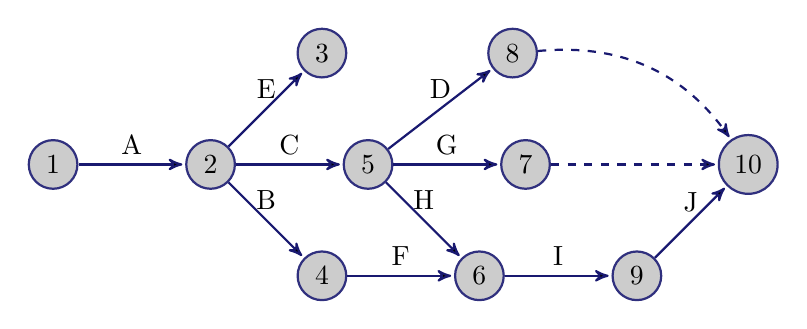
\begin{tikzpicture}[->,>=stealth',shorten >=2pt,
			line width=0/5pt, node distance=2cm]
			\node[roundnode] (one) {1};
			\node[roundnode] (two) [right of=one] {2};
			\node[roundnode] (three) [above right of=two] {3};
			\node[roundnode] (four) [below right of=two] {4};
			\node[roundnode] (five) [right of=two] {5};
			\node[roundnode] (six) [right of=four] {6};
			\node[roundnode] (seven) [right of=five] {7};
			\node[roundnode] (eight) [above right of=five, xshift=12pt] {8};
			\node[roundnode] (nine) [right of=six] {9};
			\node[roundnode] (ten) [above right of=nine] {10};
			\path[pt] (one) edge node [above] {A} (two);
			\path[pt] (two) edge node [above] {B} (four);
			\path[pt] (two) edge node [above] {C} (five);
			\path[pt] (five) edge node [above] {D} (eight);
			\path[pt] (two) edge node [above] {E} (three);
			\path[pt] (four) edge node [above] {F} (six);
			\path[pt] (five) edge node [above] {G} (seven);
			\path[pt] (five) edge node [above] {H} (six);
			\path[pt] (six) edge node [above] {I} (nine);
			\path[pt] (nine) edge node [above] {J} (ten);
			\path[pt] [dashed] (seven) edge node [above] {} (ten);
			\path[pt] [dashed] (eight) edge [bend left] node [above] {} (ten);
		\end{tikzpicture}
	\end{figure}
	
	\part Values at terminal nodes by $m$ estimator; \\
	(3) = 6 \\
	(10) via (4) = 11.5 \\
	(10) via (5) = 13.5 \\
	(7) = 13 \\
	(8) = 10 \\
	
	\textbf{Summary: }
	The critical path is A-C-H-I-J with a most-likely time of 13.5 days.
	
	\part
	Showtime = June 30; 99\% confidence $\rightarrow z=2.33$ \\
	\begin{tabular}{ccccc|ccc}
		Activity & Pred & $a$ & $b$ & $m$ & $E$(*) & Var(*) &  \\ \midrule
		   A     &  —   &  2  &  4  &  3  &   3    &  1/9   &  \\
		   B     &  A   &  1  &  3  &  2  &   2    &  1/9   &  \\
		   C     &  A   &  2  & 10  &  6  &   6    & 1 7/9  &  \\
		   D     &  C   &  1  &  3  &  2  &   2    &  1/9   &  \\
		   E     &  A   &  1  &  5  &  3  &   3    &  4/9   &  \\
		   F     &  B   &  2  &  4  &  3  &   3    &  1/9   &  \\
		   G     &  C   &  3  &  7  &  5  &   5    &  4/9   &  \\
		   H     &  C   & 0.5 & 1.5 &  1  &   1    &  1/36  &  \\
		   I     & F,H  &  1  &  2  & 1.5 &  1.5   &  1/36  &  \\
		   J     &  I   &  1  &  3  &  2  &   2    &  1/9   &  \\
	\end{tabular} \\

	\textbf{CP}: \(E(T_{1,2}+T_{2,5}+T_{5,6}+T_{6,9}+T_{9.10}) = 13.5\) \\
	\(\text{Var}(T_{1,2}+T_{2,5}+T_{5,6}+T_{6,9}+T_{9.10}) = 2\frac{1}{18}\)
	\[0.99=P(z\leq2.33)=P(CP\leq13.5+(2\frac{1}{3})(2\frac{1}{18})=18.2962)\]

	
	\textbf{Summary: }
	The preparations for the concert should begin no later than mid-day on June 11, if the promoter does not take any time off. 
	If however, the promoter is in a union and has weekends off they should start on June 2nd, unless the concert is on a Saturday or Sunday, in which case they should start June 1st or May 13st respectively. \\
	In either case, this schedule provides a 99\% probability of meeting the deadline, based on the information provided.
	
	\part%
	The following LP could be used to find the critical path for this project:
	\begin{flalign*}
		\text{Min } z=x_{10}-x_1 & & \\
		\text{s.t.} \qquad \qquad \quad
		x_2 &\geq x_1 + 3 & \\ 
		x_3 &\geq x_2 + 3 & \\ 
		x_4 &\geq x_2 + 2 & \\ 
		x_5 &\geq x_2 + 6 & \\ 
		x_6 &\geq x_4 + 3 & \\
		x_6 &\geq x_5 + 1 & \\ 
		x_7 &\geq x_5 + 5 & \\ 
		x_8 &\geq x_5 + 2 & \\ 
		x_9 &\geq x_6 + 1.5 & \\ 
		x_{10} &\geq x_9 + 2 & \\
		x_1,x_2,x_3,x_4,x_5,&x_6,x_7,x_8,x_9,x_{10} \geq 0 & 
	\end{flalign*}
	
\end{parts}
\end{solution}


\question
Consider the following travel distance data: \\
\makebox[\linewidth]{Distance in Miles}\\
\setcellgapes{1pt}
\makegapedcells
\begin{tabularx}{\textwidth}{|c|Y|Y|Y|Y|Y|Y|}
	\hline
	\diagbox{From}{To} & 1  & 2  & 3  & 4  & 5  & 6  \\ \hline
	        1          & -  & 42 & 20 & 31 & 29 & 33 \\ \hline
	        2          & 42 & -  & 58 & 45 & 68 & 47 \\ \hline
	        3          & 20 & 58 & -  & 28 & 32 & 51 \\ \hline
	        4          & 31 & 45 & 28 & -  & 57 & 61 \\ \hline
	        5          & 29 & 68 & 32 & 57 & -  & 34 \\ \hline
	        6          & 33 & 47 & 51 & 61 & 34 & -  \\ \hline
\end{tabularx} \\

\begin{parts}
	\part%
	Use the nearest neighbor heuristic (it is just what it sounds like), starting with a depot at 1 to provide a sequence for the traveling salesman problem where you must visit each city only once and return to the depot. Be sure to give the total distance with your sequence.
	
	\part%
	Discuss the pros and cons of this approach
	
\end{parts}

\begin{solution}
\begin{parts}
	\part%
	\begin{tabular}{l|c|l}
		Visited & Dist. & Remaining \\
		1 & 0 & 2,3,4,5,6 \\
		1,3 & 20 & 2,4,5,6 \\
		1,3,4 & 48 & 2,5,6 \\
		1,3,4,2 & 93 & 5,6 \\
		1,3,4,2,6 & 140 & 5 \\
		1,3,4,2,6,5 & 174 & \\
		1,3,4,2,6,5,1 & 203 & \\
	\end{tabular}
	
	\textbf{Summary: }
	Using the plain nearest-neighbor algorithm, the salesman will travel from node 1 to 3,4,2,6,5, in that order, and finally back to 1. During this route the salesman will travel 203 miles.
	
	\part%
	The nearest neighbor algorithm is a heuristic with all the pros and cons of a greedy algorithm. Specifically, it is fast, simple, requires very few calculations, is easy for a human to do, and likely to give a significantly better than random answer. The primary downside is that it is not unlikely that the result will be suboptimal. In some cases, especially with larger and more complex networks the suboptimality is likely to grow significantly.
	
\end{parts}
\end{solution}


\end{questions}
\end{document}